\documentclass[12pt,prb,aps,epsf]{article}
\usepackage[utf8]{inputenc}
\usepackage{amsmath}
\usepackage{amsfonts}
\usepackage{amssymb}
\usepackage{graphicx} 
\usepackage{latexsym} 
\usepackage[toc,page]{appendix}
%\usepackage{listings}
\usepackage{xcolor}
\usepackage{soul}
\usepackage[T1]{fontenc}
\usepackage{amsthm}
\usepackage{mathtools}
\usepackage{setspace}
\usepackage{array,multirow,makecell}
\usepackage{geometry}
\usepackage{textcomp}
\usepackage{float}
\usepackage{cancel}
\usepackage{here}
\usepackage{titlesec}
\usepackage{bbold}

\geometry{hmargin=2cm,vmargin=2cm}

\begin{document}
	
	\title{LP 48 Phénomènes de résonance dans différents domaines de la physique}
	\author{Naïmo Davier}
	\date{Agrégation 2018}
	
	\maketitle
	
	\tableofcontents
	
	\pagebreak
	
\subsection{Introduction}
Prérequis : mécanique, MQ, ondes, électromag...

Exemples usuels : casser un verre avec sa voix, ponts qui s'écroule lorsqu'on marche au pas....ect

On va essayer d'en faire une définition plus générale dans cette leçon.

\section{Résonance à 1 DDL : RLC}
Commençons par regarder le cas d'un oscillateur (amorti) usuel : le RLC.\\
\begin{figure}[h]
	\centering 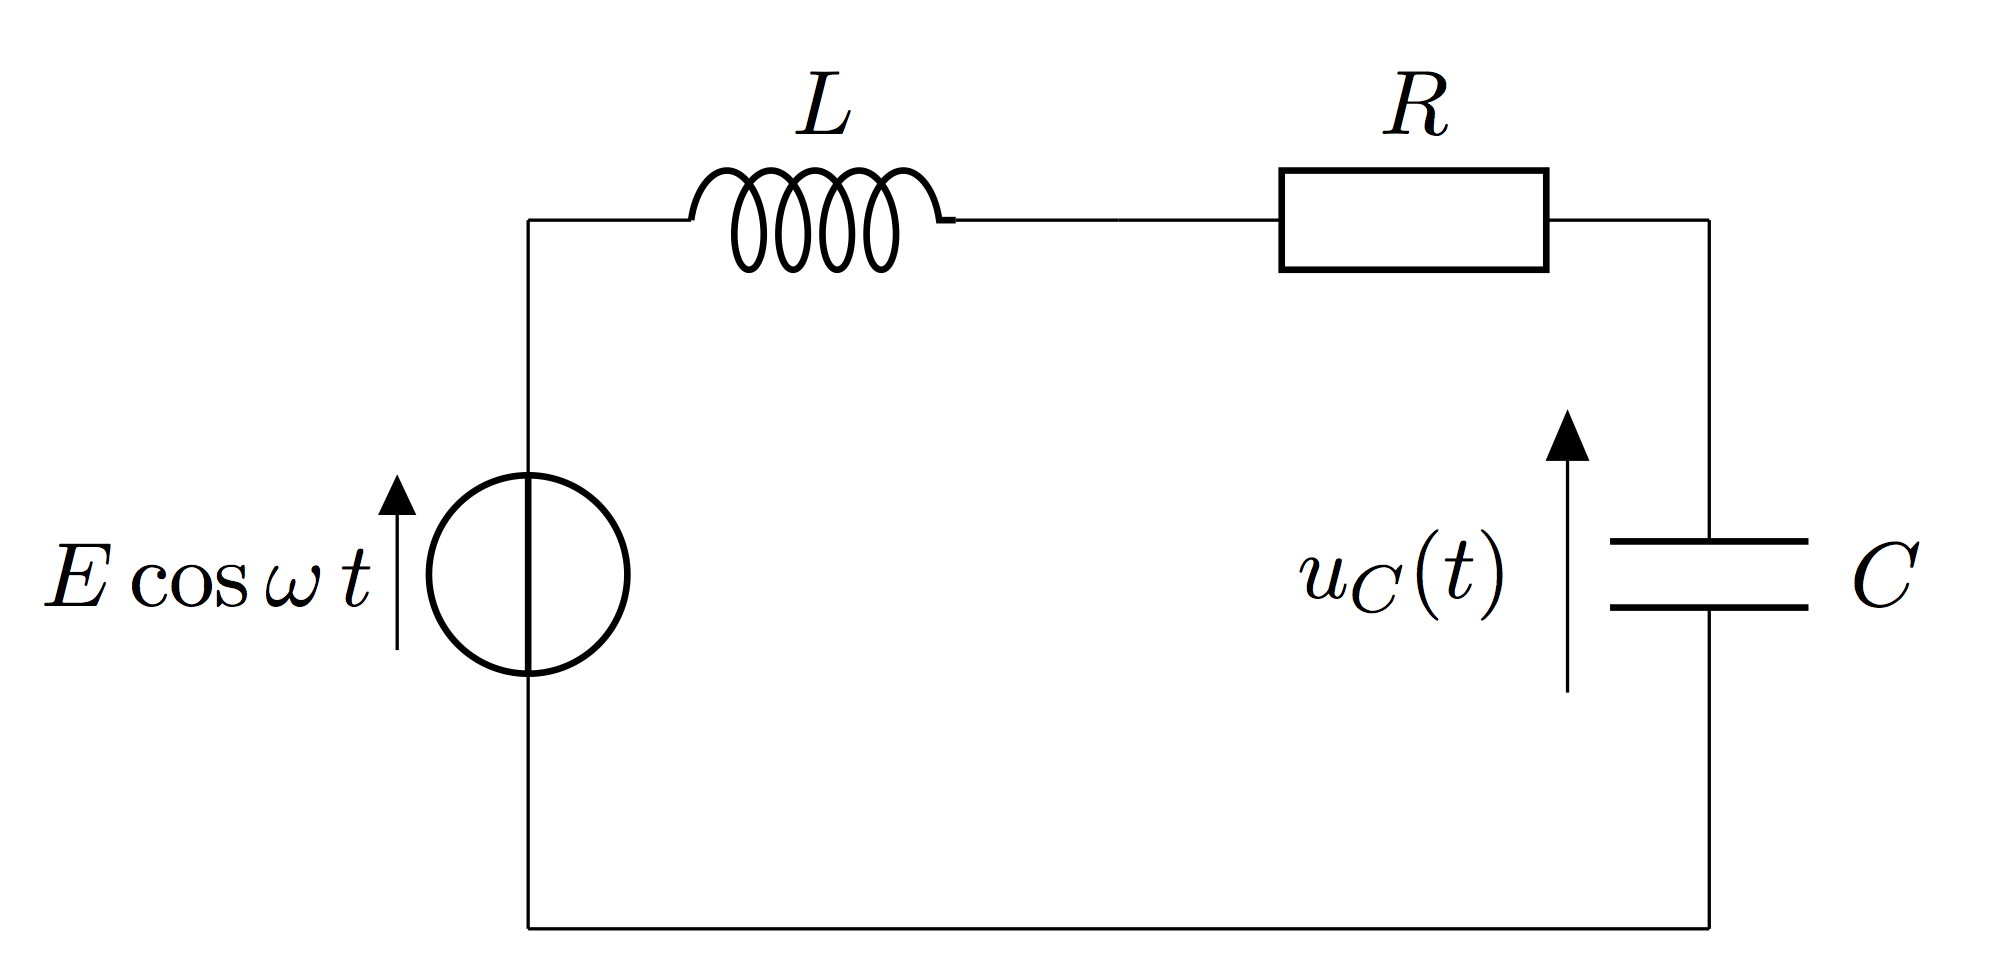
\includegraphics[width=10cm]{RLC}
\end{figure}
On applique la loi des mailles dans le cas où on a un GBF délivrant une tension sinusoïdale $e(t) = E\cos(\omega t)$ pour obtenir
\begin{eqnarray}
L\frac{d i}{dt} + Ri + \frac{1}{C}q = e(t)\\
\frac{d^2q}{dt^2} + \frac{1}{\tau}\frac{dq}{dt} + \omega_0^2q = \frac{e(t)}{L}
\end{eqnarray}
avec $\tau = L/R$ et $\omega_0^2 = \frac{1}{LC}$. Cette équation différentielle est en fait assez générale et s'applique à plusieurs système, sa résolution et les conclusions qu'on en tire sont donc applicables à plus que le RLC. Le forçage étant sinusoïdal et l'équation étant linéaire on passe en complexe et on cherche une solution de la forme $\underline{q}(t) = \underline{A}e^{i\omega t}$ (cela revient à décomposer les solutions sur la base des ondes planes, qui est base propre des opérateurs différentiels), on obtient alors 
\begin{eqnarray}
\left(-\omega ^2 + \frac{i\omega}{\tau} + \omega_0^2\right) \underline{A} = \frac{E}{L}
\end{eqnarray}
ce qui mène à 
\begin{eqnarray}
q(t) = Re\left[\frac{Ee^{i\omega t}}{L\left(\omega_0^2-\omega ^2 + \frac{i\omega}{\tau} \right)}\right]
\end{eqnarray}
et ainsi 
\begin{eqnarray}
i(t) = Re\left[\frac{i\omega Ee^{i\omega t}}{L\left(\omega_0^2-\omega ^2 + \frac{i\omega}{\tau} \right)}\right] = \frac{\omega E}{L}\frac{\omega/\tau \cos(\omega t) - (\omega_0^2-\omega^2) \sin(\omega t) }{(\omega_0^2-\omega^2)^2 + \omega^2/\tau^2}
\end{eqnarray}
On constate alors si on trace l'amplitude de $i$ en fonction de la pulsation qu'elle admet un maximum à lorsque la pulsation du générateur est égale à la fréquence propre de l'oscillateur $\omega_0$. Ainsi la puissance aux bornes du condensateur 
\begin{eqnarray}
P = u_Ci = \frac{qi}{C} \propto \omega q^2
\end{eqnarray}
est maximale pour cette même pulsation, on parle alors de résonance puisque le transfert d'énergie entre le générateur et le circuit est maximal. Et dans ce cas la fréquence de résonance est donc égale à la fréquence de résonance.\\

Il est possible à ce point de définir l'admittance
\begin{eqnarray}
Y(\omega) = \frac{"vitesse"}{"Force"} = \frac{I(\omega)}{E}
\end{eqnarray}
qui une grandeur générale caractérisant bien le phénomène de résonance : à la résonance l'impact sur le système du forçage et donc l'admittance sont maximaux.\\

\textbf{Pour les docteurs : Manip : tracé de la résonance en courant : i(f) + phase}. On en déduit la fréquence de résonance du circuit.\\

On peut généraliser ce phénomène de résonance aux oscillateurs ayant plus d'un degrés de liberté comme nous allons maintenant le voir.

\section{Résonance dans les les systèmes à plusieurs DDL}
\subsection{2 OH couplés}
On regarde la cas de deux oscillateurs couplés : deux masses identiques sont liées entre elles et à deux supports verticaux à l'aide de 3 ressorts (le tout est à l'horizontale). Cela peut modéliser par exemple la molécule de $CO_2$ : $O=C=O$ où les liaisons covalentes peuvent êtres vues comme deux puits de potentiels et donc approximables par deux oscillateurs harmoniques.\\

\begin{figure}[h]
	\centering 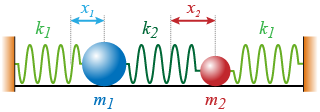
\includegraphics[width=10cm]{osc_couples}
\end{figure}
On voit en appliquant le PFD que l'on a un système de deux équations couplées pour les position des deux masses
\begin{eqnarray}
m\ddot{x}_1 = -kx_1 + k_2(x_2-x_1)\\
m\ddot{x}_2 = -kx_2 - k_2(x_2-x_1)
\end{eqnarray}
que l'on peut réécrire sous forme matricielle 
\begin{eqnarray}
m
\begin{pmatrix}
\ddot{x}_1\\
\ddot{x}_2
\end{pmatrix}
= \begin{pmatrix}
- k - k_2& k\\
k & - k - k_2
\end{pmatrix}
\begin{pmatrix}
x_1\\
x_2
\end{pmatrix}
\end{eqnarray}
équivalent à l'équation type 
\begin{eqnarray}
\ddot{\vec{X}} + \omega_0^2 M\vec{X} = 0
\end{eqnarray}
où
\begin{eqnarray}
M = \begin{pmatrix}
1+\varepsilon & -\varepsilon\\
- \varepsilon & 1+ \varepsilon
\end{pmatrix}
\hspace{1cm}\mathrm{avec}\hspace{1cm} \omega_0^2 = \frac{k_2}{m}\;\;\mathrm{et}\;\; \varepsilon = \frac{k}{k_2}
\end{eqnarray}
La matrice M est diagonalisable, on peut donc la diagonaliser puis effectuer un changement de base afin de se placer dans la base propre du système dans laquelle apparaîtront deux oscillateurs découplés et donc indépendants. Commençons par diagonaliser $M$, pour cela on commence par chercher les valeurs propres en résolvant 
\begin{eqnarray}
\det(M - \lambda \mathbb{1}) = 0\\
\Rightarrow\; (1+\varepsilon-\lambda)^2 &=& \varepsilon^2\\
1 + \varepsilon - \lambda &=& \pm \varepsilon\\
\Rightarrow\;\;\lambda_1 = 1\hspace{1cm}\mathrm{et}\hspace{1cm}\lambda_2 = 1+2\varepsilon
\end{eqnarray}
Ce qui signifie que les deux fréquences propres du systèmes sont $\omega_1 = \omega_0$ et $\omega_2 = (1+2\varepsilon)\omega_0$ où $\omega_0$ est la fréquence propre d'un oscillateur seul (avec un ressort de raideur $k_2$).\\
On peut maintenant chercher les vecteurs propres $\vec{y}_1$ et $\vec{y}_2$ de $M$, commençons par $\vec{y}_1 = \begin{pmatrix}
\alpha_1\\ \beta_1
\end{pmatrix}$ tel que $M\vec{y}_1 = \vec{y}_1$ ce qui équivaut à
\begin{eqnarray}
(1+\varepsilon)\alpha_1 - \varepsilon \beta_1 = \alpha_1\\
\Leftrightarrow \alpha_1 = \beta_1
\end{eqnarray}
On a donc $\vec{y}_1 = \frac{1}{\sqrt{2}}\begin{pmatrix}
1\\ 1
\end{pmatrix}$ ce que l'on peut formuler comme $y_1(t) = \frac{1}{\sqrt{2}}(x_1(t) + x_2(t))$. Si on fait de même pour $\vec{y}_2$ on trouve $y_2(t) = \frac{1}{\sqrt{2}}(x_1(t) - x_2(t))$.\\ Géométriquement le premier mode correspond au cas $y_2(t)=0$ et donc $x_1(t) = x_2(t)$, les deux masses oscillent alors en phase, le ressort central ayant une longueur constamment égale à sa longueur à vide. Le second mode correspond quant à lui à $y_1(t) = 0$ et ainsi $x_1(t) = -x_2(t)$ : mode antisymétrique où les deux masses oscillent en opposition de phase.\\

De même que pour le cas à 1DDL précédent on va exciter le système de manière résonante si on force une des deux masse à vibrer à une des deux fréquences propre du système. Ainsi pour la molécule de $CO_2$ on observe deux raies d'absorptions correspondant à ces deux modes : lorsque la fréquence de l'onde incidente est égale à l'une des deux fréquences de résonance on a un transfert maximal d'énergie à la molécule : il y a absorption.\\ 

Le raisonnement que l'on vient d'effectué est tout a fait généralisable aux cas où on a plus de 2 oscillateurs couplés, on aura dans le cas général N oscillateurs couplés qui mèneront à N équations différentielles couplées. On aura ainsi une matrice $N\times N$ à diagonaliser, nous donnant N modes propres. Les modes propres pouvant êtres définis comme un "mouvement collectif indépendant à une fréquence propre dans lequel les composantes entretiennent des relations d'amplitude et de phase". Les N fréquences associées conduiront alors à l'apparition d'un phénomène de résonance à chaque fois que l'on excitera le système à l'une de ses fréquences propres.\\

Regardons maintenant ce qu'il se passe lorsque le nombre d'oscillateurs devient très grand. 

\subsection{N OH couplés}
On regarde le cas d'un standard d'un cristal unidimensionnel constitué d'atomes identiques liés par des ressorts identiques. Question : quels sont les modes propres d'un tel système ? On note $x_p$ la position du $p^{ieme}$ atome, et $\omega_i$ la pulsation du $i^{eme}$ mode propre. Pour ce mode propre tous les atomes $x_p$ oscillent alors à la même pulsation $\omega_i$, avec l'amplitude $x_p^i$ et la phase $\phi_p^i$. Le nombre d'atomes couplés étant très grand, on le considère comme infini, on a alors invariance par translation ce qui signifie que l'on a 
\begin{eqnarray}
x_p^i = x_0^i\;\; \forall p\\
\phi^i_{p+1} - \phi^i_p = \Delta \phi_0^i = k^ia
\end{eqnarray}
et donc $\phi_p^i = \phi_0^i + p(k^ia) = \phi_0^i + k^i(pa)$. Cela nous amène finalement à 
\begin{eqnarray}
x_p^i(t) = x_0^i e^{j(k^ipa - \omega_i t)}
\end{eqnarray}
on voit donc que les modes propres se présentent sous la forme d'onde plane.\\
Il reste à savoir comment exprimer le déphasage $\Delta \phi_0^i=k^ia$ en fonction de la pulsation du mode auquel elle est attachée : c'est la relation de dispersion. Pour cela on regarde l'équation du mouvement 
\begin{eqnarray}
m\ddot{x}_p = -k(x_p-x_{p-1}) + k(x_{p+1}-x_p)
\end{eqnarray}
dans laquelle on injecte la forme que l'on vient de déterminer 
\begin{eqnarray}
-m\omega_i^2x_p^i &=& - 2kx_p^i + k x_{p-1}^i + k x_{p+1}^i \\
&=& x_p^i (-2k + k e^{-jk^ia} + ke^{jk^ia})\\
\Rightarrow -m\omega_i^2 &=& 2k (\cos(k^ia)-1)\\
&=& -4k\sin^2\frac{k^ia}{2}
\end{eqnarray}
On obtient donc finalement la relation de dispersion
\begin{eqnarray}
w_i = 2\omega_0 \left|\sin\frac{k^ia}{2}\right|
\end{eqnarray}
 La question centrale ici est : Quels sont les modes propres permis (pour lesquels on aura donc résonance) ?\\
 
 Cela va dépendre des conditions au limite qui vont conduire à une quantification modes permis. Si on prend un cristal de longueur $L=Na $ avec Cl périodiques $x_0(t) = x_N(t)$ on a ainsi $e^{jkNa} = 1$ et donc $k^i = \frac{2\pi}{L} i$. Le mode fondamental correspond alors à $k^0=0$ : tous les atomes sont en phase, c'est une mode complètement symétrique et on peut résonner de même pour les autres modes.\\
 
  On constate ici que ce sont cette fois les $CL$ qui fixent les fréquences pour les quelles il va y avoir résonance.\\
  
 On constate ici que pour les grandes longueur d'onde on a  l'impression de voir une onde se propager, on peut donc se demander ce qu'il se passe lorsqu'on fait tendre la taille caractéristique des oscillateurs $a$ vers 0.
\subsection{Passage au continu}
Pour les grandes longueur d'onde on a $k^ia\ll1$ et le mouvement est alors constitué d'un ensemble de mouvement individuels $\{x_p(t)\}$ : N fonctions du temps, le système est donc compliqué à décrire. On peut alors construire un objet plus simple : une fonction qui interpole tous les points et qui dépend donc cette fois de deux variables $\psi(x,t)$ telle que $\psi(x=pa,t) = x_p(t)$. On a ainsi construit une fonction lisse qui passe par tous les points réels. Si on suppose que la fonction construite est au moins $\mathcal{C}^2$ on alors 
\begin{eqnarray}
\ddot{x}_p + \omega_0^2 (2x_p - x_{p+1} - x_{p-1}) = 0
\end{eqnarray}
qui devient 
\begin{eqnarray}
\frac{\partial^2 \psi}{\partial t^2} + \omega_0^2 ((x_p-x_{p-1}) -(x_{p+1}-x_p)) = 0\\
 \frac{\partial^2 \psi}{\partial t^2} + \omega_0^2 [(\psi(pa,t)-\psi(pa-a,t)) - (\psi(pa+a,t)-\psi(pa,t))] =0\\
 \frac{\partial^2 \psi}{\partial t^2} + a\omega_0^2 \left(\frac{\partial \psi}{\partial x} (x-a,t) -\frac{\partial \psi}{\partial x} (x,t) \right) = 0\\
 \frac{\partial^2 \psi}{\partial t^2} - a^2\omega_0^2\frac{\partial^2 \psi}{\partial x^2} (x,t) = 0
\end{eqnarray}
on constate que l'on vient d'établir l'équation de d'Alembert 
\begin{eqnarray}
\Delta \psi(x,t) - \frac{1}{c^2}\frac{\partial^2 \psi}{\partial t^2} = 0
\end{eqnarray}
avec $c=a\omega_0$ la célérité des ondes dans le cristal continu. La relation de dispersion est alors $\omega = ck$, ce qui correspond au cas du cristal dans la limite $a\rightarrow0$.\\

On constate là encore que ce sont les $CL$ qui vont fixer les modes propres puisque sans conditions limites toutes les fréquences sont permises.
\section{Résonance avec C.L}
\subsection{Corde de Melde}
\begin{figure}[h!]
	\centering 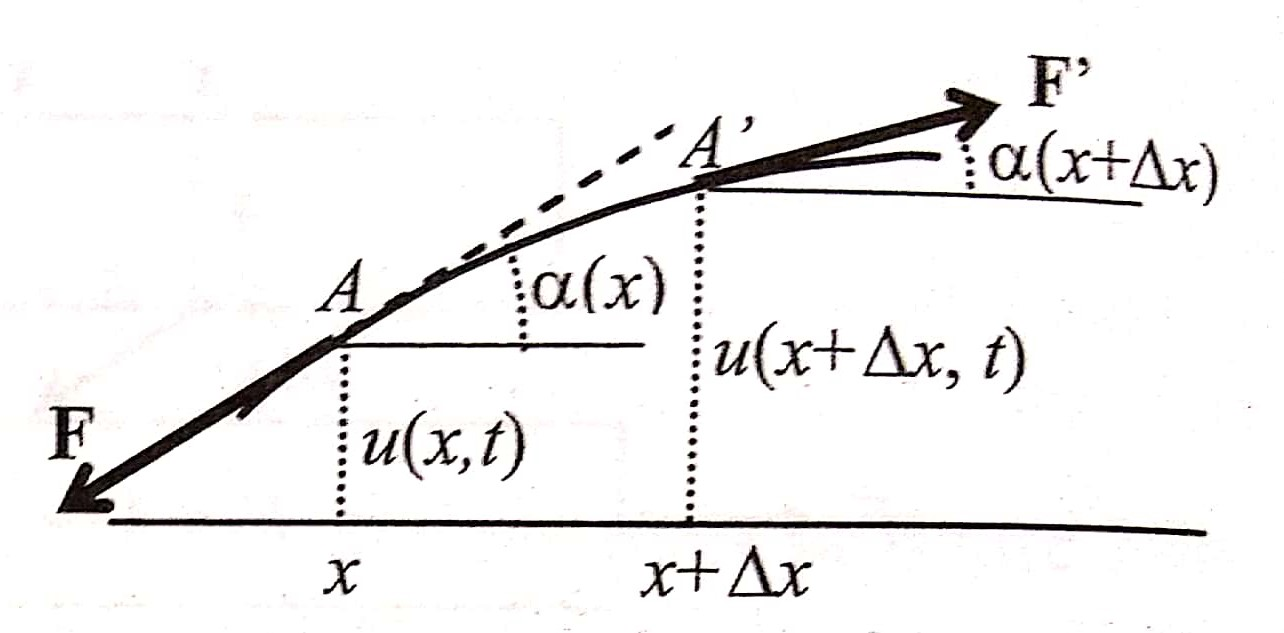
\includegraphics[width=8cm]{corde_schema}
	\centering 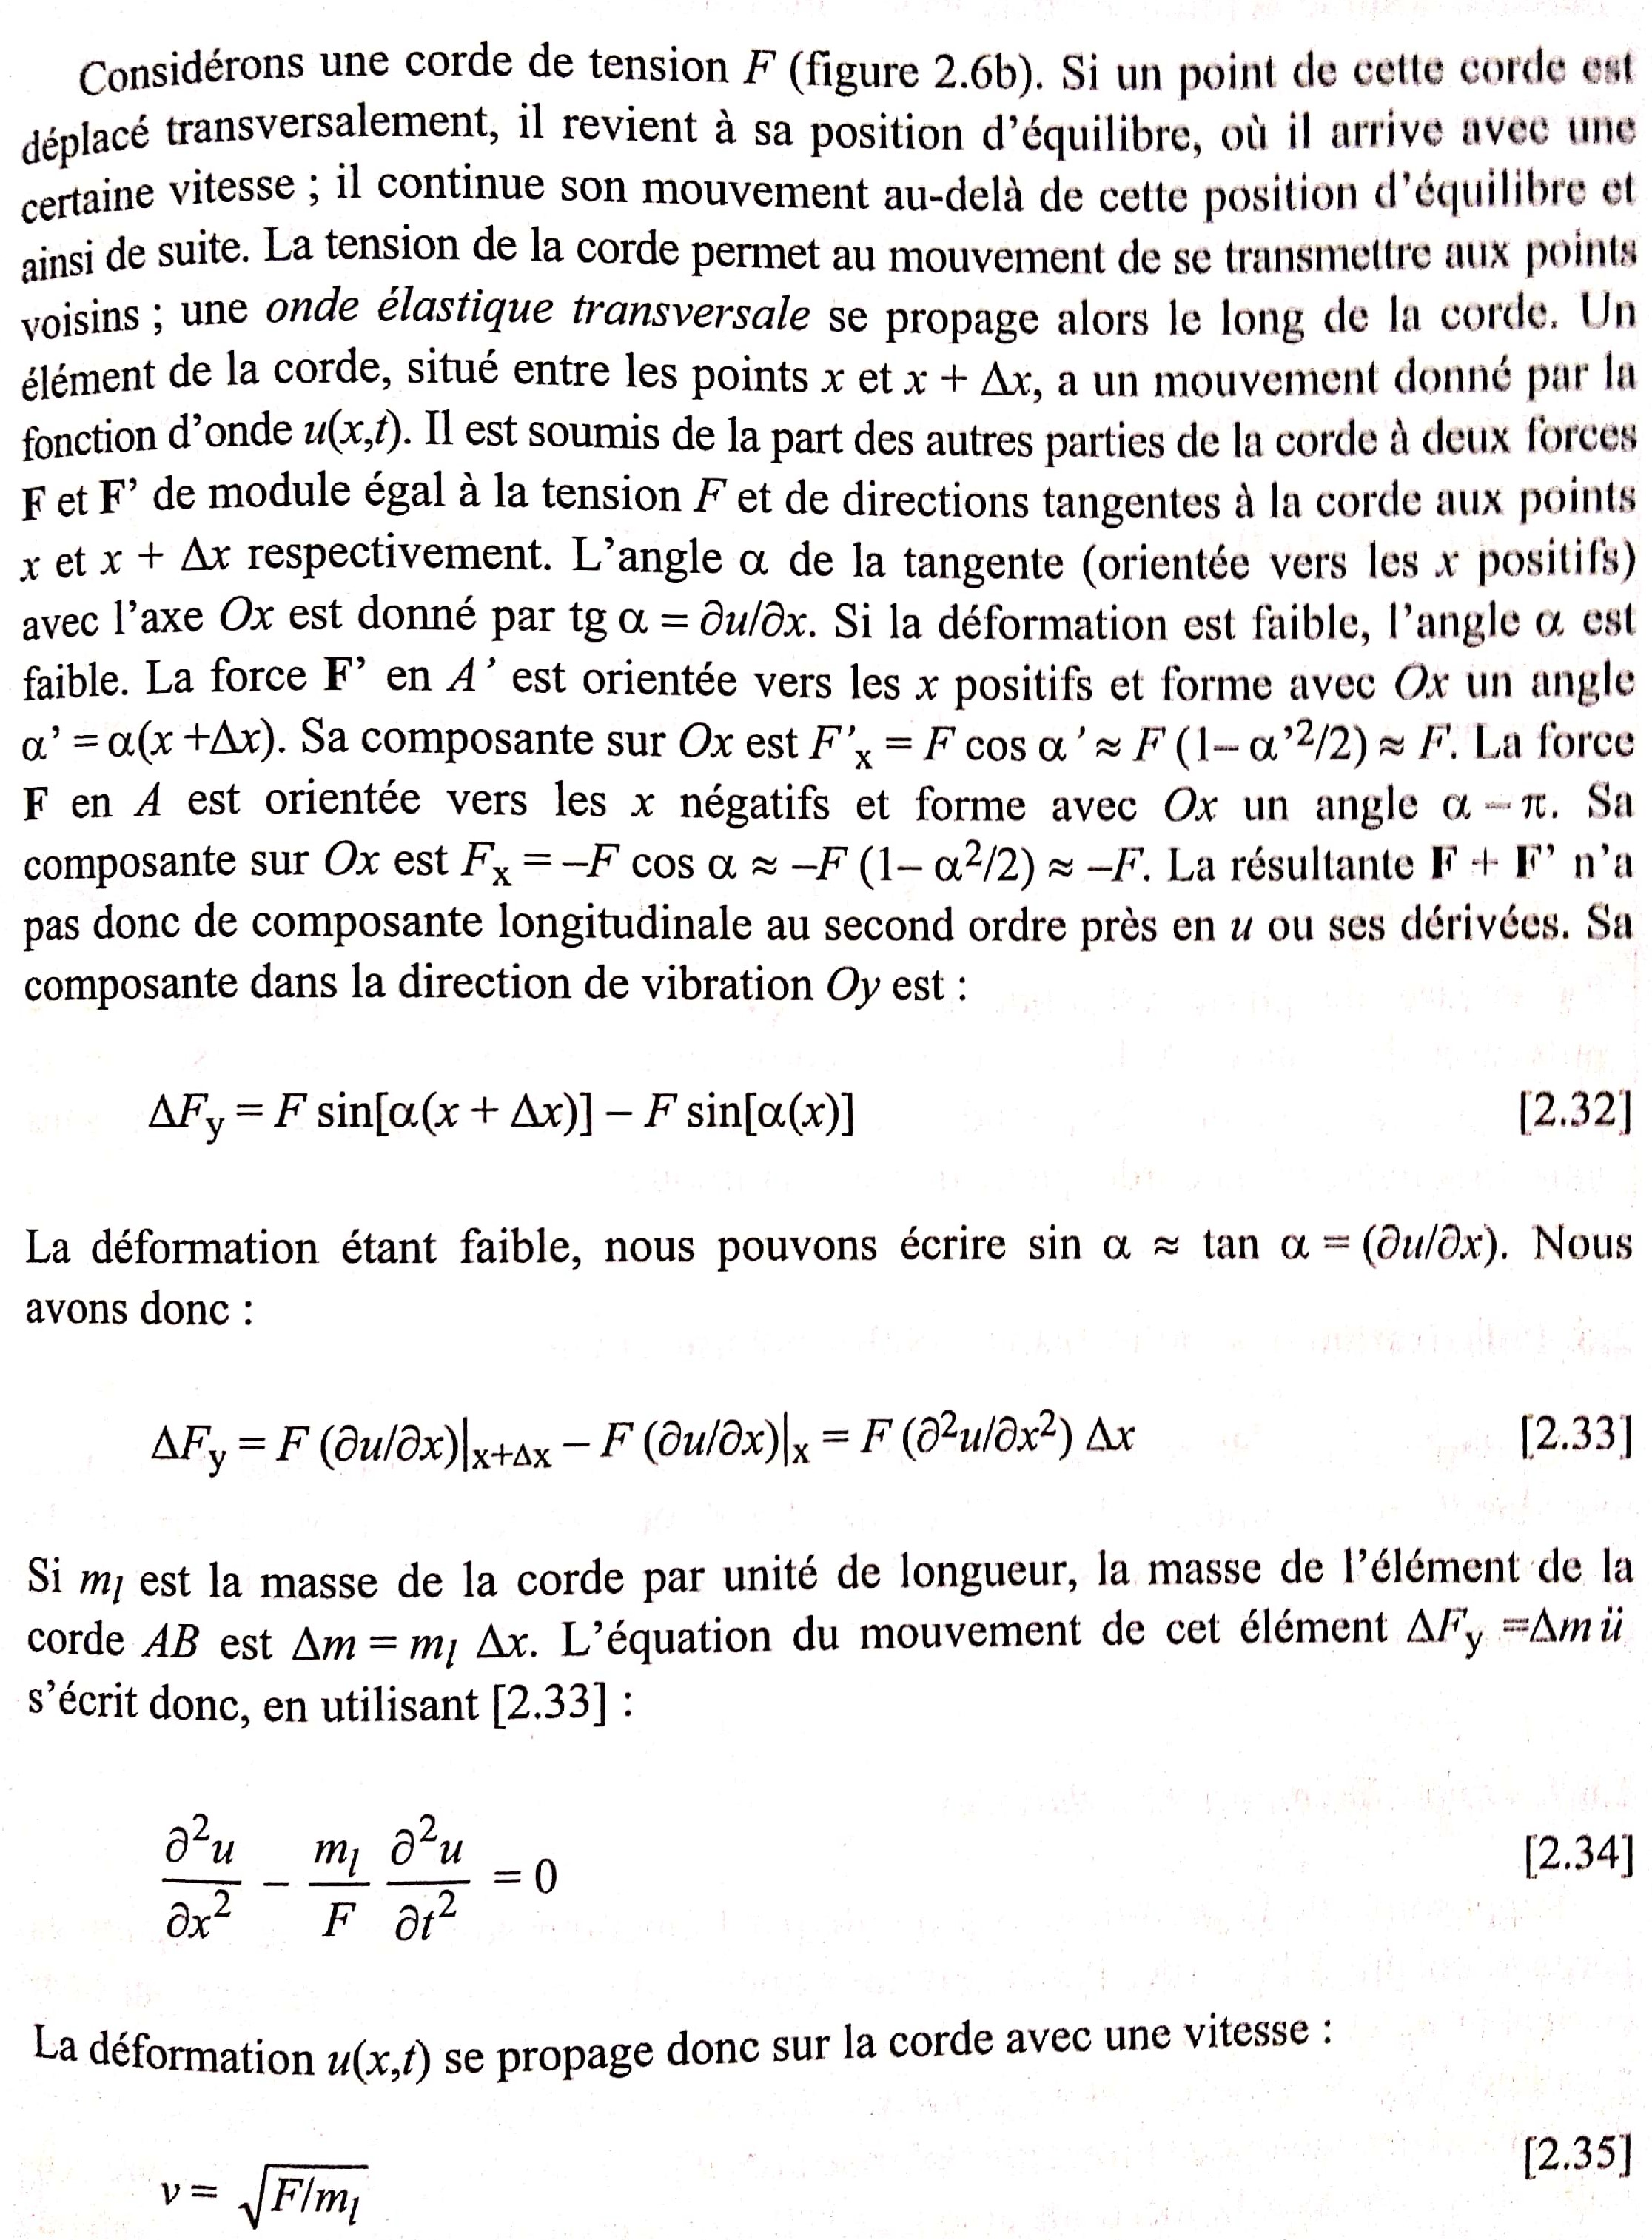
\includegraphics[width=14.2cm]{corde}
\end{figure}

Description générale... on arrive à l'équation de D'Alembert (sans faire les calculs) avec la vitesse $c = \sqrt{\frac{T}{\mu}}$.\\

Les conditions limites sont imposées par un nœud de vibration d'un coté, et une excitation sinusoïdale de l'autre. Elles vont conduire à des fréquences propres discrètes étant celles pour lesquelles ondes incidente et réfléchie se superposent pour interférer constructivement.

On a donc une onde plane, et une divergence apparente lorsque sin(kL) = 0, à savoir lorsque $L= p\frac{\lambda}{2}$ ou de manière équivalente $\omega = p \frac{\pi c }{L}$ : forçage résonant. 

\subsection{Fabry Pérot}
\textbf{Pérez d'optique}\\
On constate un phénomène similaire mais avec cette fois une onde lumineuse et non une onde de déplacement matérielle. Le phénomène est similaire : l'onde incidente et l'onde réfléchie interfèrent constructivement lorsqu'on est à la résonance.

\section{Puits de potentiel en MQ}
\subsection{Puits $\infty$}
\textbf{Paragraphe 8.3.3 p262 Le Bellac tome I}

\subsection{Calcul de Bohr et de De Broglie pour l'hydrogène}
\textbf{modèle de Bohr p36 Le Bellac Tome I}\\
$2\pi r_n = n\lambda_{dB}$ : atome = onde électronique dans une boite.

\section{Conclusion}
La résonance est un phénomène qui se caractérise par un transfert maximal d'énergie lorsque qu'un système est forcé à l'une de ces fréquences propres. Ces fréquences propres peuvent soient apparaître à cause de la structure d'oscillateur, soit à cause des dimensions et conditions limites imposées à une onde propagative.

\section*{Questions}
Vous parlez de l'universalité de la résonance, y a t-il résonance pour un circuit RL ou RC ?\\
Non : ce sont des systèmes du premier ordre, et seuls les systèmes d'ordre deux au moins peuvent êtres résonants.\\

Est ce donc universel ?\\
NON.\\

Dans quels types de systèmes ce phénomène se manifeste ?\\
Systèmes oscillants : systèmes d'ordre 2 ou plus.\\

Concernant la barrière de potentiel en MQ, dans quel cas rencontre on cette situation ?\\
Microscope à effet tunnel.\\

Vous dites qu'il y a résonance lorsque la largeur de la barrière est liée à la fréquence de l'onde incidente... et vous nous parlez d'électron, quelle est la fréquence d'un électron ?\\

Vous pouvez établir d'Alembert dans le cas de la corde ?\\

Prendre une excitation sinusoïdale ou en cosinus fait il une différence ?\\
Non cela correspond juste à un choix arbitraire de l'origine des temps.\\

Pouvez vous donner le lien entre vitesse et transfert d'énergie ?\\
C'est la puissance.

\section*{Remarques}
Il faut maitriser toutes les démos sur lesquelles on passe vite, ou qu'on passe sous silence.\\
Il faut introduire la notion de base des ondes planes : base propre des opérateurs différentiels linéaires.\\
On doit bien montrer que Fabry-Pérot = Corde de Melde : dans les deux cas on a $p\lambda = 2L$ : l'onde se superpose alors à elle même en phase. Mais du coup il faut vite passer sur le second présenté.\\
Il faut expliciter la relation de dispersion à chaque fois : montre la différence entre d'Alembert et Schrodinger ! En MQ le vide est dispersif !!\\
Impédance : $Z = \frac{U}{I} = \frac{"Force"}{"vitesse"}$ et admittance $Y = \frac{I}{U}$.\\
Résonance : puissance reçue maximale. Si on trace $P(\omega)$ on a un max à la fréquence de résonance. C'est donc la résonance en puissance qui est universelle.\\

Résonance bien faite dans le Pérez de Mécanique.\\

Il faut bien introduire la fréquence propre : on a résonance lorsqu'on excite le système à sa fréquence de résonance.\\

On peut citer plusieurs cas de systèmes plus exotiques : Drude Lorrentz, vibrations moléculaires : il faut expliciter le fait que c'est la même physique : oscillateur harmonique universel car correspond aux petites oscillations dans un puits de potentiel.\\

Analogie possible sur les systèmes en rotation avec le théorème du moment cinétique : RMN et RPE.\\

Dans le cas oscillateurs couplés citer la molécule $CO_2$ et prendre deux ressorts identiques de part et d'autre. Passer par la forme matricielle pour introduire les modes propres. Elargir en disant que les deux modes propres obtenus sont généraux car les équations sont linéaires. Dans le cas du $CO_2$ on a donc deux raies d'absorption.\\
Tous les systèmes de taille finies se ramènent donc à une diagonalisation : généralisable au cas de N oscillateurs.\\
On enchaine alors sur le passage au continu. Mais quand on arrive à d'Alembert la résonance n'est plus évidente .... toutes les fréquences sont possibles, il y a une infinité de modes propres dans le vide. Cette fois la résonance vient des conditions limites.\\


\end{document}